\documentclass[border=10pt]{standalone}

\usepackage{tikz}
\usepackage{tikzsymbols}
\usetikzlibrary{calc,patterns,shapes.geometric}

\def\centerarc[#1](#2)(#3:#4:#5){\draw[#1] ($(#2)+({#5*cos(#3)},{#5*sin(#3)})$) arc (#3:#4:#5);}

\begin{document}
	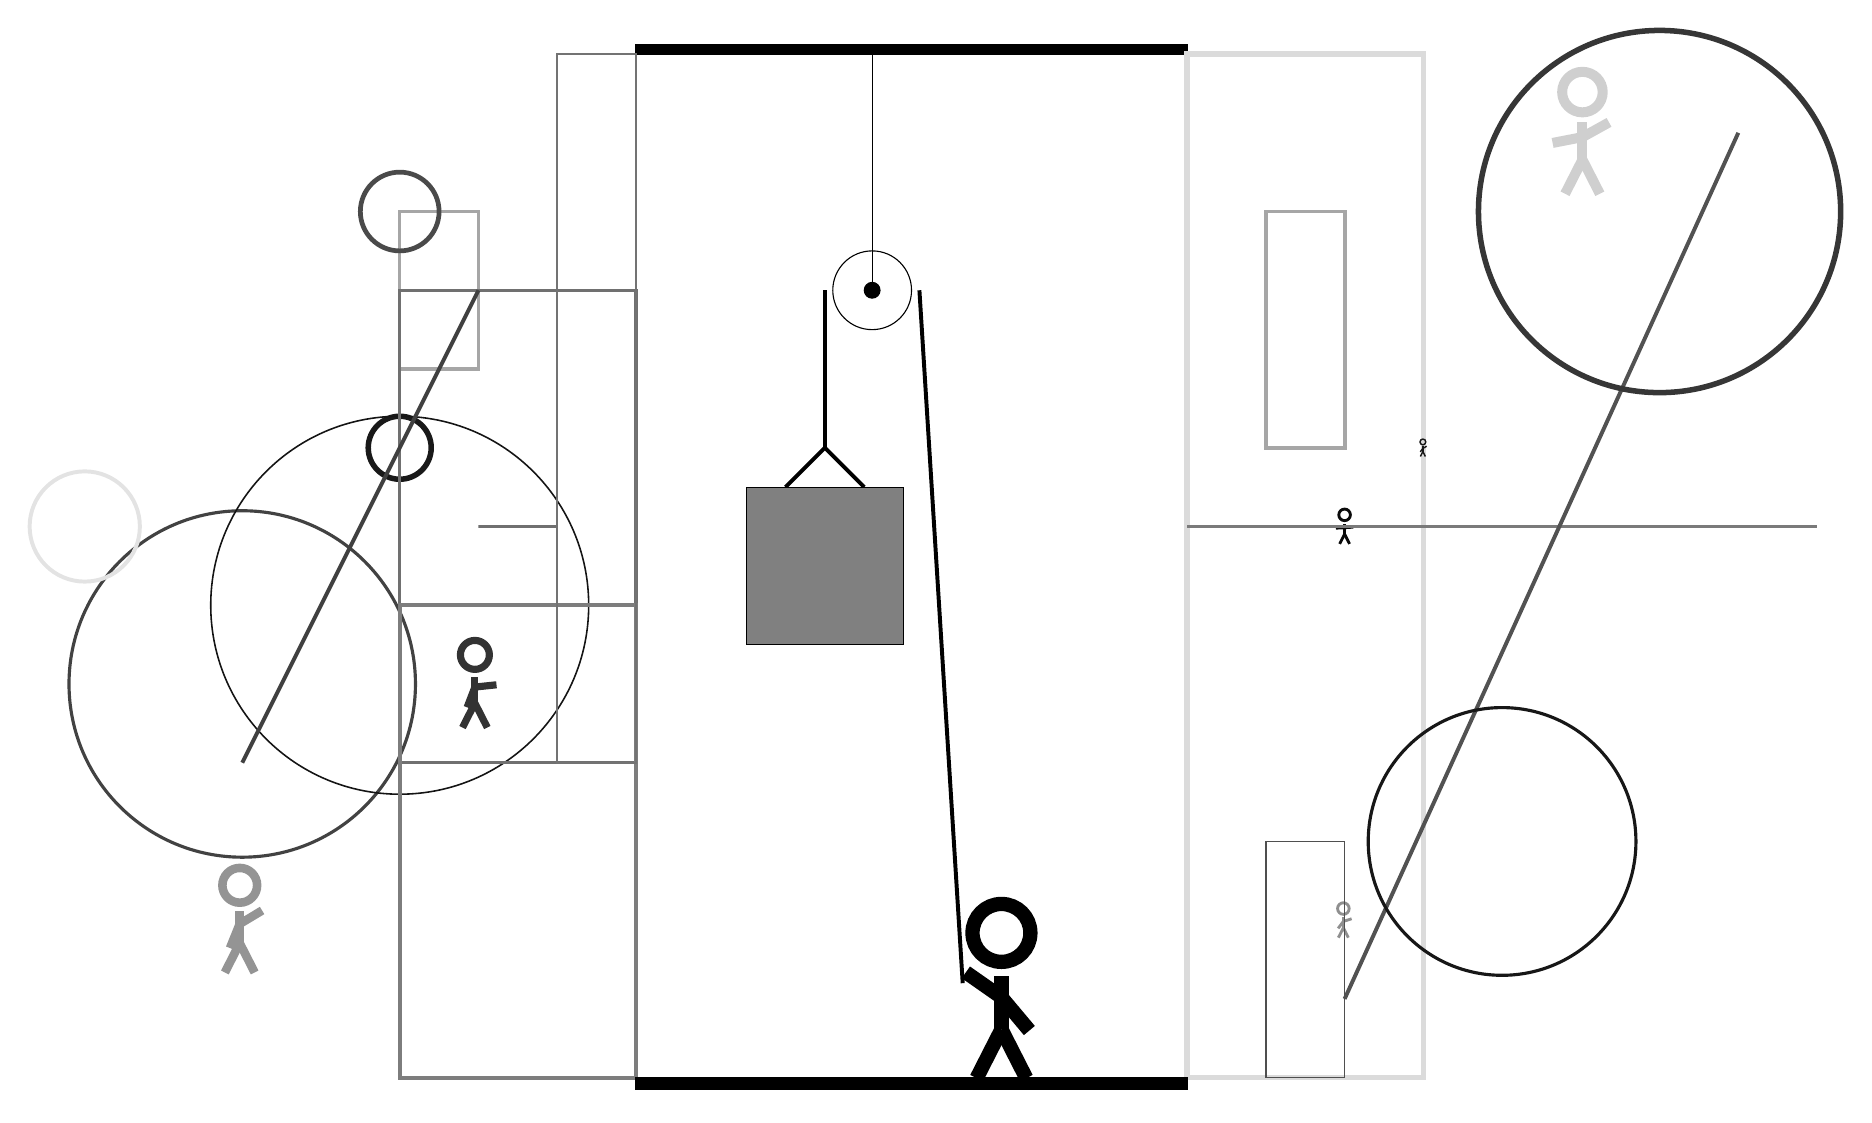
\begin{tikzpicture}
		%%%%% START %%%%%
		
		\draw[fill=black] (-2, 10) rectangle (5, 10.125);
		
		\draw (1, 7) circle (0.5);
		\draw[fill=black] (1, 7) circle (0.1);
		\draw (1, 10) -- (1, 7);
		
		\draw[line width=0.5mm] (-0.1, 4.5) -- (0.4, 5.0) -- (0.9, 4.5);
		\draw[fill=black!50] (-0.6, 4.5) rectangle (1.4, 2.5);
		
		\node[line width=0.4mm, color=black!19] at (10, 9) {\Strichmaxerl[7][11][29]};
		
		\node[line width=0.5mm, color=black!96] at (7, 4) {\Strichmaxerl[2][3][4]};
		\draw [line width=0.7mm, color=black!90](-5, 5) circle (0.4);
		\draw[line width=0.4mm, color=black!35] (-4, 6) rectangle (-5, 8);
		
		\node[line width=0.2mm, color=black!42] at (-7, -1) {\Strichmaxerl[6][68][31]};
		\draw[line width=0.7mm, color=black!14] (5, -3) rectangle (8, 10);
		
		\draw [line width=0.4mm, color=black!74](-7, 2) circle (2.2);
		
		\draw [line width=0.6mm, color=black!71](-5, 8) circle (0.5);
		\node[line width=0.2mm, color=black!44] at (7, -1) {\Strichmaxerl[2][53][18]};
		\draw[line width=0.5mm, color=black!52](5, 4) -- (13, 4);
		
		\draw [line width=0.2mm, color=black!92](-5, 3) circle (2.4);
		\draw[line width=0.5mm, color=black!68](7, -2) -- (12, 9);
		\draw[line width=0.4mm, color=black!56] (-2, 1) rectangle (-5, 7);
		\draw[line width=0.5mm, color=black!35] (7, 5) rectangle (6, 8);
		\draw [line width=0.4mm, color=black!91](9, 0) circle (1.7);
		\draw[line width=0.5mm, color=black!51] (-2, 3) rectangle (-5, -3);
		\draw[line width=0.2mm, color=black!69] (6, 0) rectangle (7, -3);
		\draw[line width=0.5mm, color=black!75](-4, 7) -- (-7, 1);
		\draw [line width=0.7mm, color=black!79](11, 8) circle (2.3);
		\node[line width=0.6mm, color=black!90] at (8, 5) {\Strichmaxerl[1][53][29]};
		\node[line width=0.5mm, color=black!80] at (-4, 2) {\Strichmaxerl[5][69][6]};
		\draw[line width=0.4mm, color=black!56] (-3, 4) rectangle (-4, 4);
		\draw[line width=0.3mm, color=black!55] (-3, 10) rectangle (-2, 1);
		\draw [line width=0.5mm, color=black!11](-9, 4) circle (0.7);
		
		\draw[line width=0.5mm] (0.4, 7) -- (0.4, 5.0);
		\centerarc[line width=0.5mm](1, 7)(0:180:0.6);
		\draw[line width=0.5mm](1.6, 7) -- (2.15, -1.8);
		
		\node at (2.6, -1.9) {\Strichmaxerl[10][-35][-50]};
		
		\draw[fill=black] (-2, -3) rectangle (5, -3.15);
		
		%%%%% END %%%%%
	\end{tikzpicture}
\end{document}